\documentclass[10pt]{extarticle}

%Paquetes utilizados en esta tarea
\usepackage{logo}
\usepackage{enumerate}
\usepackage{fullpage}
\usepackage[utf8]{inputenc}
\usepackage[spanish]{babel}
\usepackage{epsfig}
\usepackage{amsmath}
\usepackage{amssymb}
\usepackage{epstopdf}
\usepackage[hidelinks]{hyperref}
\usepackage{algorithmic}
\usepackage[nothing]{algorithm}
\usepackage{listings}
\usepackage{color}

\definecolor{dkgreen}{rgb}{0,0.5,0}
\definecolor{dkblue}{rgb}{0,0,0.5}
\definecolor{gray}{rgb}{0.5,0.5,0.5}
\definecolor{purple}{rgb}{0.4,0,0.4}

\lstset{frame=tb,
  language=Java,
  aboveskip=3mm,
  belowskip=3mm,
  showstringspaces=false,
  columns=flexible,
  basicstyle={\small\ttfamily},
  numbers=none,
  numberstyle=\tiny\color{dkblue},
  keywordstyle=\color{dkblue},
  commentstyle=\color{gray},
  stringstyle=\color{dkgreen},
  breaklines=true,
  breakatwhitespace=true,
  tabsize=3
}
%Definiciones de comandos, para reutilizar secuencias frecuentes o ahorrar
% c�digo
\newcommand{\RR}{\mathbb{R}}
\newcommand{\lb}{\\~\\}
\newcommand{\la}{\leftarrow}

\newcommand{\twopartdef}[4]
{
	\left\{
		\begin{array}{ll}
			#1 &  \text{si }#2 \\
			#3 &  \text{si }#4
		\end{array}
	\right.
}

\newcommand{\threepartdef}[6]
{
	\left\{
		\begin{array}{ll}
			#1 &  \text{si }#2 \\
			#3 &  \text{si }#4 \\
			#5 &  \text{si }#6
		\end{array}
	\right.
}

\makeatletter

\makeatother

\begin{document}

\begin{tabular}{ccl}
\begin{tabular}{c}
\psfig{file=puclogo.eps}
\end{tabular}
&\ \ \ & 
\begin{tabular}{l}
PONTIFICIA UNIVERSIDAD CATÓLICA DE CHILE\\
ESCUELA DE INGENIERÍA\\
DEPARTAMENTO DE CIENCIAS DE LA COMPUTACIÓN\\
MECOLAB
\end{tabular}
\end{tabular}

\begin{center}
\bf Andrés Matte Vallejos\\
\bf matte.andres@gmail.com\\
\bf 1er semestre del 2015\lb

\vspace{0.5cm}

\bf {\Huge Tutorial Sync Adapter}
\end{center}

\tableofcontents

\newpage

\section{Introducción}

\paragraph{}
Mantener una aplicación móvil no sincronizada con la web la vuelve prácticamente inservible. Hoy en día es difícil pensar en una aplicación importante que no descargue o suba datos a algún servidor. Claramente este feature hace que una aplicación luzca más profesional y da una mejor experiencia de usuario. Por ejemplo a un usuario de Facebook le gustaría que un cambio de foto de perfil no solo se realice en la web, si no que también ocurra en todos sus dispositivos móviles.

\paragraph{}
Hay muchas formas de realizar una sincronización de datos con un servidor. Si bien cada desarrollador puede implementar su propio sistema, no hay necesidad de reinventar la rueda. O en este caso, para qué vamos a reinventar algo mucho más complejo que una rueda: un Sync Adapter. Este framework ayuda a manejar y automatizar las transferencias de datos.


\subsection{Beneficios}

\begin{enumerate}
 \item Ejecución automatizada: la sincronización estará definida de acuerdo a tu configuración y se ejecutará automáticamente de acuerdo a eso. Con esto podemos eliminar el botón de refresh.
 \item Revisión de conectividad: por ejemplo, si en algún momento no hay conexión a internet y corresponde una sincronización el framework se encargará de realizar la sincronización nuevamente cuando la haya.
 \item Encolación de transferencias fallidas: si se está descargando un archivo y esto falla, se vuelve a intentar.
 \item Gasta menos batería: muchas veces el framework realizará la sincronización de más de una aplicación al mismo tiempo. De esta forma la radio se enciende con menor frecuencia.
 \item Centralización de la transferencia: la sincronización de los datos se realiza toda al mismo tiempo y en el mismo lugar.
 \item Manejo de cuenta y autenticación: si el usuario de tu aplicación requiere credenciales especiales se puede integrar el manejo de cuentas y autenticación en la transferencia.
\end{enumerate}

\subsection{Qué haremos}

\paragraph{}
Durante el siguiente tutorial se utilizará una aplicación sencilla que liste a los integrantes de un curso. Se podrá añadir estudiantes, tanto en el servidor web como en la aplicación android, y se deberán mantener sincronizados los datos a través de un sync adapter. No se entrará en temas que escapan del objetivo del tutorial como el servidor, las vistas o sobre como se realizan los requests. De todas formas en \url{https://github.com/aamatte/ListaAlumnosAndroid} se puede revisar el código de la aplicación utilizada para los ejemplos\footnote{Algunos detalles en el código pueden variar en el tiempo pero los conceptos serán los mismos}.


\subsection{Qué se necesita}

\paragraph{}
Para que el Sync Adapter esté funcionando necesitamos implementar seis componentes, donde cada una juega un papel importante:

\begin{enumerate}
 \item Base de datos
 \item Content Provider
 \item Authenticator
 \item Clase Sync Adapter
 \item Bound Service
\end{enumerate}



\section{Base de datos}

\paragraph{}
En android se pueden guardar información de diferentes maneras, pero en este caso utilizaremos bases de datos. Usaremos SQLite, el sistema por defecto para android. En esta parte del tutorial no se ahondará de sobremanera debido a que es un tema transversal y hay mucha documentación al respecto.

\subsection{Qué haremos}

\begin{enumerate}
 \item Definir un esquema y sus constantes
 \item Crear base de datos y tablas
 \item Crear métodos CRUD
\end{enumerate}

\subsection{Definir un esquema y sus constantes}

\paragraph{}
Una vez que el modelo relacional esté definido este se debe plasmar en una clase que llamaremos DatabaseContract. Esta tendrá definidas como String los nombres de las tablas, de las columnas y algunas operaciones importantes. Gracias a esto podemos cambiar el nombre de, por ejemplo, una columna sin la necesidad de cambiar el resto de nuestro código.

\begin{lstlisting}
// DatabaseContract.java
public final class DatabaseContract {

    public DatabaseContract() {
    }

    public static abstract class Students implements BaseColumns {
		// BaseColumns nos entrega las constantes _ID y _COUNT
		
        public static final String TABLE_NAME = "STUDENTS";
        public static final String COLUMN_NAME_STUDENT_NAMES = "names";
        public static final String COLUMN_NAME_FIRST_LASTNAME = "firstlastname";
        public static final String COLUMN_NAME_SECOND_LASTNAME = "secondlastname";
        public static final String COLUMN_ID_CLOUD = "idcloud";

        public static final String TEXT_TYPE = " TEXT";
        public static final String INTEGER_TYPE = " INTEGER";
        public static final String COMMA_SEP = ",";

        public static final String SQL_CREATE_STUDENTS_TABLE =
                "CREATE TABLE " + Students.TABLE_NAME + " (" +
                        Students._ID + " INTEGER PRIMARY KEY," +
                        Students.COLUMN_NAME_STUDENT_NAMES + TEXT_TYPE + COMMA_SEP +
                        Students.COLUMN_NAME_FIRST_LASTNAME + TEXT_TYPE + COMMA_SEP +
                        Students.COLUMN_NAME_SECOND_LASTNAME + TEXT_TYPE + COMMA_SEP+
                        Students.COLUMN_ID_CLOUD + INTEGER_TYPE +
                        " )";

        public static final String SQL_DELETE_STUDENTS =
                "DROP TABLE IF EXISTS " + Students.TABLE_NAME;
    }
}
\end{lstlisting}

\subsection{Crear base de datos y tablas}

\paragraph{}
Ahora utlizaremos la clase SQLiteOpenHelper, una API para poder interactuar con nuestra base de datos. Cuando utilizas esta clase el sistema realiza las operaciones de larga duración cuando tu lo decidas y no en el inicio de la aplicación. Lo único que se debe hacer es llamar a $getWritableDatabase()$ o a $getReadableDatabase()$. 
\paragraph{}
Las instancias de SQLiteDatabase retornadas por estos métodos están especialmente configuradas para realizar las operaciones especificadas. Esto quiere decir que $getWritableDatabase()$ retornará una instancia en el que la escritura de datos será rápida en desmedro de la lectura. Con $getReadableDatabase()$ no se podrá escribir y tendrá una lectura más rápida. Además, al llamar a estos métodos se crea la base de datos en caso de no existir aún.

\paragraph{}
Otro método escencial es $onCreate(SQLiteDatabase)$. Ahí es donde se ejecuta el código SQL para crear las tablas de la base de datos. También están $onUpgrade(SQLiteDatabase)$ y $onDowngrade(SQLiteDatabase)$.

\begin{lstlisting}
// StudentsDbHelper.java
// Documentacion:
// http://developer.android.com/reference/android/database/sqlite/SQLiteOpenHelper.html
import android.content.Context;
import android.database.sqlite.SQLiteDatabase;
import android.database.sqlite.SQLiteOpenHelper;

public class StudentsDbHelper extends SQLiteOpenHelper {

    public static final int DATABASE_VERSION = 1;
    public static final String DATABASE_NAME = "Students.db";

    private static StudentsDbHelper sInstance;

    private StudentsDbHelper(Context context) {
        super(context, DATABASE_NAME, null, DATABASE_VERSION);
    }
	
	// Nos aseguramos de que solo haya una instancia para evitar errores.
	// Mas detalles: 
	// http://www.androiddesignpatterns.com/2012/05/correctly-managing-your-sqlite-database.html
    public static synchronized StudentsDbHelper getInstance(Context context) {
        if (sInstance == null) {
            sInstance = new StudentsDbHelper(context.getApplicationContext());
        }
        return sInstance;
    }
	
    @Override
    public void onCreate(SQLiteDatabase db) {
        db.execSQL(DatabaseContract.Students.SQL_CREATE_STUDENTS_TABLE);
    }
	
	// Cambia la version del esquema en caso de haber modificaciones.
	// Por simplicidad asumimos que esto no va a pasar y tan solo se resetea la db.
    @Override
    public void onUpgrade(SQLiteDatabase db, int oldVersion, int newVersion) {
        db.execSQL(DatabaseContract.Students.SQL_DELETE_STUDENTS);
        onCreate(db);
    }
}
\end{lstlisting}

\paragraph{}
Para tener acceso a la base de datos se debe hacer lo siguiente:
\begin{lstlisting}
StudentsDbHelper mDbHelper = StudentsDbHelper.newInstance();
SQLiteDatabase db = mDbHelper.getWritableDatabase();
\end{lstlisting}
O en el otro caso:
\begin{lstlisting}
StudentsDbHelper mDbHelper = StudentsDbHelper.newInstance();
SQLiteDatabase db = mDbHelper.getReadableDatabase();
\end{lstlisting}

\subsection{Crear métodos CRUD}

\subsubsection{Agregar datos}
\paragraph{}
Para insertar datos se deben ingresar los datos del elemento a añadir en ContentValues y usar el método insert. El segundo argumento especifica la columna en que la base de datos puede puede insertar null si values (los datos a ingresar) está vacio. Si es que no quieres que se ingrese un record con valores vacios debes setearlo como null. Por ejemplo, si se quiere añadir un estudiante:
	
\begin{lstlisting}
// Codigo para insertar nuevo estudiante

if (mDbHelper == null) {
    mDbHelper = StudentsDbHelper.getInstance(getActivity());
}
SQLiteDatabase db = mDbHelper.getWritableDatabase();

ContentValues values = new ContentValues();
values.put(DatabaseContract.Students.COLUMN_NAME_STUDENT_NAMES, student.getNames());
values.put(DatabaseContract.Students.COLUMN_NAME_FIRST_LASTNAME, student.getFirstLastname());
values.put(DatabaseContract.Students.COLUMN_NAME_SECOND_LASTNAME, student.getSecondLastname());
values.put(DatabaseContract.Students.COLUMN_ID_CLOUD, student.getIdCloud());

// Retorna la columna en la que fue insertado
long success = db.insert(
        DatabaseContract.Students.TABLE_NAME, 
        null,								  
        values);
        
if (success >= 0) return true;
return false;
     
\end{lstlisting}

\subsubsection{Consultar datos}
\paragraph{}
Para esto se usa el método query(). Si no se quiere filtrar y solo obtener toda la información de la tabla se pueden dejar todos los valores como null excepto el nombre de la tabla. Para seleccionar todos los estudiantes:

\begin{lstlisting}
// Codigo para seleccionar todos los estudiantes

if (mDbHelper == null) {
    mDbHelper = StudentsDbHelper.getInstance(getActivity());
}

// Selecciono las columnas que debe retornar de cada fila. Podria dejarse como null y me retorna todas.
String[] projection = {DatabaseContract.Students.COLUMN_NAME_STUDENT_NAMES,
                       DatabaseContract.Students.COLUMN_NAME_FIRST_LASTNAME,
                       DatabaseContract.Students.COLUMN_NAME_SECOND_LASTNAME,
                       DatabaseContract.Students.COLUMN_ID_CLOUD
                       };

// Se deja como null porque no se requiere filtrar. Por ejemplo, si se necesitara filtrar por primer apellido:
// String selection = DatabaseContract.Students.COLUMN_NAME_FIRST_LASTNAME + "= ?"
String selection = null;

// Que el primer apellido sea Perez:
// String[] selectionArgs = new String[]{ "Perez" };
// En este caso dejamos como null
String[] selectionArgs = null;

SQLiteDatabase db = mDbHelper.getReadableDatabase();

Cursor c = db.query(DatabaseContract.Students.TABLE_NAME,   // Tabla
                    projection,                             // Columnas a retornar
                    selection,                              // Columnas de WHERE
                    selectionArgs,                          // Valores de WHERE
                    null,                                   // Group by
                    null,                                   // Filtro por columnas de grupos
                    DatabaseContract.Students.COLUMN_NAME_FIRST_LASTNAME +" ASC"); // Ordenados

ArrayList<Student> studentsInDb = new ArrayList<Student>();

c.moveToFirst();

if (c.getCount()<1){
    return false;
}

while (c.moveToNext()){
    String names = c.getString(c.getColumnIndexOrThrow(DatabaseContract.Students.COLUMN_NAME_STUDENT_NAMES))
    		    .toUpperCase();
    String firstLast = c.getString(c.getColumnIndexOrThrow(DatabaseContract.Students.COLUMN_NAME_FIRST_LASTNAME))
    		    .toUpperCase();
    String secondLast = c.getString(c.getColumnIndexOrThrow(DatabaseContract.Students.COLUMN_NAME_SECOND_LASTNAME))
    			.toUpperCase();
    int idCloud = c.getInt(c.getColumnIndexOrThrow(DatabaseContract.Students.COLUMN_ID_CLOUD));
    
    studentsInDb.add(new Student(names, firstLast, secondLast, idCloud));
}
     
\end{lstlisting}

\subsubsection{Borrar datos}
\paragraph{}
Se utiliza el método delete.

\subsubsection{Actualizar datos}
\paragraph{}
Se utiliza el método update.


\section{Content Provider}

\paragraph{}
Un content provider es exactamente lo que su nombre dice, un proveedor de contenido o de datos. Ofrece un esquema estructurado para acceder, crear, borrar o actualizar los datos que se pongan a disposición a través de él. En definitiva es la forma en que tu aplicación ofrece sus datos para que puedan ser consumidos o editados por procesos externos a ella o por otras aplicaciones sin la necesidad de que esta esté abierta.

\paragraph{}
Se pueden usar incluso como una forma de abstraer la implementación de un sistema de datos complejo frente al resto de los desarrolladores de una misma aplicación. De esta forma el resto de los integrantes del equipo solo deben estar al tanto de los estándares de comunicación con el content provider y no necesitan preocuparse de detalles de la implementación. De todas formas su principal objetivo es compartir los datos con otros procesos.

\subsection{Qué haremos}
\paragraph{}
En esta sección cubriremos los siguientes temas:
\begin{enumerate}
	\item Funcionamiento general
	\item Content URIs
	\item Clase Contrato
	\item Clase Content Provider
	\item Cómo utilizar el Content Provider
	\item Permisos
\end{enumerate}

\subsection{Funcionamiento general}

\paragraph{}
Como se aprecia en la Figura~\ref{fig:flujo_content_provider} el flujo parte desde tu aplicación obteniendo una instancia de ContentResolver\footnote{ContentResolver: http://developer.android.com/reference/android/content/ContentResolver.html}. Luego, a través de esta se hace una consulta pasando como primer parámetro una URI que hace referencia a un conjunto de datos que ofrece un content provider específico. Es importante saber que pueden haber muchos content providers disponibles, cada uno con su conjunto de URIs (corresponde un URI para cada conjunto de datos ofrecido en el provider). Por ejemplo, android provee Contacts Provider\footnote{Contacts provider: http://developer.android.com/guide/topics/providers/contacts-provider.html} y Calendar Provider\footnote{Calendar provider: http://developer.android.com/guide/topics/providers/calendar-provider.html}. En la próxima sección se entrará más en detalles en el diseño de las URIs.

\paragraph{}
Nuestra instancia de ContentResolver decide a qué provider hacer la consulta basado en la URI. Luego el content provider determina a qué conjunto de datos debe afectar (también basado en la URI) e interactúa con la base de datos para realizar la operación que fue invocada.
\begin{figure}[H]
    \centering
    \includegraphics[width=0.8\textwidth]{ContentProviderGeneral.png}
    \caption{Flujo general de content provider}
    \label{fig:flujo_content_provider}
\end{figure}



\subsection{Content URIs}

\paragraph{}
Un content URI es un identificador de un conjunto de datos en un provider. Está formado por el identificador del provider (authority) y por un nombre que indica a la tabla o al contenido que hace referencia. Cuando se llama a un método para acceder a algún conjunto de datos se debe incluir en los parámetros una URI determinada. Esto para que el ContentResolver pueda determinar a qué provider le corresponde manejar el llamado, y para que el provider pueda determinar sobre que datos realizar la operación.

\begin{figure}[H]
    \centering
    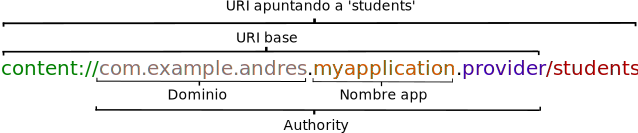
\includegraphics[width=0.8\textwidth]{provider_uri_explicacion.png}
    \caption{Estructura content URI}
    \label{fig:estructura_content_URI}
\end{figure}



\subsubsection{Authority}

\paragraph{}
La authority es el identificador de tu aplicación dentro de android. Por lo general el formato de este viene dado por el package de la aplicación más 'provider'. Por ejemplo, en el caso de nuestra aplicación es \textit{com.example.andres.myapplication.provider}. En el package (y en este caso, en la authority) se suele utilizar como primeras palabras un dominio de internet, al revés, al cual pertenece la aplicación. En este caso asumimos que hay un dominio con la ruta \textit{andres.example.com}.

\subsubsection{Estructura de rutas URI}

\paragraph{}
Para el content provider se puede diseñar una estructura nueva de los datos de acuerdo a lo que se quiera ofrecer. En la clase contrato definiremos nuevas tablas (que pueden ser iguales a las de tu base de datos o no) que conformarán la estructura de rutas. En nuestro caso solo definiremos una tabla Students igual a la de nuestra base de datos. Claramente se pueden hacer estructuras más complejas con tablas anidadas y más esoterismos, pero no se cubrirán en este tutorial\footnote{Para más detalles mirar: \url{http://developer.android.com/guide/topics/providers/content-provider-creating.html\#ContentURI}}.

\paragraph{}
Para nuestra aplicación definiremos dos URIs, una para obtener la lista completa de estudiantes y otra para obtener a un estudiante en particular basandonos en su ID. La primera es exactamente como la que está en la Figura~\ref{fig:estructura_content_URI}. La segunda debe poder soportar llamados del tipo 
\begin{center}
\textit{content://com.example.andres.myapplication.provider/students/3},
\end{center}
donde 3 es el id del estudiante a seleccionar. Para poder soportar esto debemos definir la URI de la siguiente manera:

\begin{center}
\textit{content://com.example.andres.myapplication.provider/students/\#}
\end{center}


\subsection{Clase Contrato}

\paragraph{}
La clase contrato es la que contiene todos los URIs, MIME Types y constantes necesarias para poder tener un protocolo de comunicación fijo entre los distintos procesos que utilizan el provider. Esta clase es la que debes compartir con otros desarrolladores si quieres que usen tu provider, ya que con ella les proveerás todos las valores necesarios para que se puedan comunicar con él de manera correcta. Básicamente, en la aplicación que utilice el provider se debe copiar y pegar la clase contrato.

\paragraph{}
A continuación se presenta el código de la clase contrato de nuestra aplicación de ejemplo. Los conceptos involucrados se explicarán luego.

\begin{lstlisting}

import android.content.ContentResolver;
import android.net.Uri;
import android.provider.BaseColumns;

/**
 *  Esta clase provee las constantes y URIs necesarias para trabajar con el StudentsProvider
 */
public final class StudentsContract {

    public static final String AUTHORITY = "com.example.andres.myapplication.provider";
    public static final Uri BASE_URI = Uri.parse("content://" + AUTHORITY);
    public static final Uri STUDENTS_URI = Uri.withAppendedPath(StudentsContract.BASE_URI, "/students");

    /*
        MIME Types
        Para listas se necesita  'vnd.android.cursor.dir/vnd.com.example.andres.provider.students
        Para items se necesita 'vnd.android.cursor.item/vnd.com.example.andres.provider.students'
        La primera parte viene esta definida en constantes de ContentResolver
     */
    public static final String URI_TYPE_STUDENT_DIR = ContentResolver.CURSOR_DIR_BASE_TYPE +
            "/vnd.com.example.andres.provider.students";

    public static final String URI_TYPE_STUDENT_ITEM = ContentResolver.CURSOR_ITEM_BASE_TYPE +
            "/vnd.com.example.andres.provider.students";

    /*
        Tabla definida en provider. Aca podria ser una distinta a la de la base de datos,
        pero consideramos la misma.
     */
    public static final class StudentsColumns implements BaseColumns{

        private StudentsColumns(){}

        public static final String NAMES = "names";
        public static final String FIRST_LASTNAME = "firstlastname";
        public static final String SECOND_LASTNAME = "secondlastname";
        public static final String ID_CLOUD = "idcloud";

        public static final String DEFAULT_SORT_ORDER = FIRST_LASTNAME + " ASC";

    }

}
     
\end{lstlisting}

\subsubsection{MIME Types}

\paragraph{}
De lo que está presente en la clase contrato y no se ha hablado es de los MIME Types. Estos conforman una manera estandar de clasificar los tipos de archivos o datos. Estos tipos son los mismos siempre, independiente del sistema operativo o de cualquier otra variante que se presente. Un MIME Type tiene dos partes: un tipo y un sub-tipo que están separados por un slash (/). Por ejemplo, las imagenes de formato JPEG tienen el MIME Type \textit{image/jpeg}.

\paragraph{}
En el caso del provider se especifican dos MIME Types principales. El primero es para items individuales, donde el tipo viene dado por \textit{\textbf{vnd.android.cursor.item}} y el subtipo (para nuestro provider) por \textit{/vnd.com.example.andres.provider.students}. El otro es para listas, donde el tipo viene dado por \textit{\textbf{vnd.android.cursor.dir}} y el subtipo (para nuestro provider) por   \textit{/vnd.com.example.andres.provider.students} (igual que para el de items individuales). De esta forma los MIME Types completos quedan como se especifica en el código.

\paragraph{}
Los MIME Types son importantes debido a que con ellas el desarrollador puede determinar el tipo de dato que se le retornará si utiliza una URI determinada en una consulta. No hay que olvidar que esta clase es principalmente un apoyo para que otros puedan utilizar los datos que les provees, por lo tanto se debe ser consistente y claro en la implementación.

\subsection{Clase Content Provider}

\paragraph{}
A continuación se creará una clase StudentProvider que herede de la clase abstracta ContentProvider. Esta obliga a implementar una serie de métodos especificados en el código que se mostrará a continuación. Por ejemplo, se pide implementar el método \textit{query}. Este método tiene el mismo nombre que el que se usa desde ContentResolver. Es decir, si llamamos a ContentResolver.query(), el content resolver determinará a qué provider llamar basado en la URI y llamará al método query() de ese provider.

\begin{lstlisting}
import android.content.ContentProvider;
import android.content.ContentValues;
import android.content.UriMatcher;
import android.database.Cursor;
import android.database.sqlite.SQLiteDatabase;
import android.net.Uri;
import android.text.TextUtils;

/*
   Clase que extiende ContentProvider y que interactua con la base de datos 
 */
public class StudentsProvider extends ContentProvider {
    public static final int STUDENT_LIST = 1;
    public static final int STUDENT_ID = 2;
    private static final UriMatcher sUriMatcher;
    static{
        sUriMatcher = new UriMatcher(UriMatcher.NO_MATCH);
        /*
            URI para todos los estudiantes.
            Se setea que cuando se pregunta a UriMatcher por la URI:
            content://com.example.andres.myapplication.provider/students
            se devuelva un entero con el valor de 1.
         */
        sUriMatcher.addURI(StudentsContract.AUTHORITY, "students", STUDENT_LIST);
        /*
            URI para un estudiante.
            Se setea que cuando se pregunta a UriMatcher por la URI:
            content://com.example.andres.myapplication.provider/students/#
            se devuelva un entero con el valor de 2.
         */
        sUriMatcher.addURI(StudentsContract.AUTHORITY, "students/#", STUDENT_ID);
    }
    /*
        Instancia de StudentsDbHelper para interactuar con la base de datos
     */
    private StudentsDbHelper mDbHelper;

    public StudentsProvider() { }

    @Override
    public boolean onCreate() {
        mDbHelper = StudentsDbHelper.getInstance(getContext());
        return true;
    }

    /*
        Llamado para borrar una o mas filas de una tabla
     */
    @Override
    public int delete(Uri uri, String selection, String[] selectionArgs) {
        SQLiteDatabase db = mDbHelper.getWritableDatabase();
        int rows = 0;
        switch (sUriMatcher.match(uri)) {
            case STUDENT_LIST:
                // Se borran todas las filas
                rows = db.delete(DatabaseContract.Students.TABLE_NAME, null, null);
                break;
            case STUDENT_ID:
                // Se borra la fila del ID seleccionado
                rows = db.delete(DatabaseContract.Students.TABLE_NAME, selection, selectionArgs);
        }
        // Se retorna el numero de filas eliminadas
        return rows;
    }

    /*
        Se determina el MIME Type del dato o conjunto de datos al que apunta la URI
     */
    @Override
    public String getType(Uri uri) {
        switch (sUriMatcher.match(uri)){
            case STUDENT_LIST:
                return StudentsContract.URI_TYPE_STUDENT_DIR;
            case STUDENT_ID:
                return StudentsContract.URI_TYPE_STUDENT_ITEM;
            default:
                return null;
        }
    }

    /*
        Inserta nuevo estudiante
     */
    @Override
    public Uri insert(Uri uri, ContentValues values) {
        SQLiteDatabase db = mDbHelper.getWritableDatabase();
        db.insert(DatabaseContract.Students.TABLE_NAME, null, values);
        return null;
    }

    /*
        Retorna el o los datos que se le pida de acuerdo a la URI
     */
    @Override
    public Cursor query(Uri uri, String[] projection, String selection,
                        String[] selectionArgs, String sortOrder) {

        SQLiteDatabase db = mDbHelper.getReadableDatabase();
        switch (sUriMatcher.match(uri)){
        
            // Se pide la lista completa de estudiantes
            case STUDENT_LIST:
                // Si no hay un orden especificado,
                // lo ordenamos de manera ascendente de acuerdo a lo que diga el contrato
                if (sortOrder == null || TextUtils.isEmpty(sortOrder)) 
                		sortOrder = StudentsContract.StudentsColumns.DEFAULT_SORT_ORDER;
                break;
                
            // Se pide un estudiante en particular
            case STUDENT_ID:
                // Se adjunta la ID del estudiante selecciondo en el filtro de la seleccion
                if (selection == null) 
                		selection = "";
                selection = selection + "_ID = " + uri.getLastPathSegment();
                break;

            // La URI que se recibe no esta definida
            default:
                throw new IllegalArgumentException(
                        "Unsupported URI: " + uri);
        }
        Cursor cursor = db.query(DatabaseContract.Students.TABLE_NAME,
                                 projection,
                                 selection,
                                 selectionArgs,
                                 null,
                                 null,
                                 sortOrder);
        // Se retorna un cursor sobre el cual se debe iterar para obtener los datos
        return cursor;
    }

    @Override
    public int update(Uri uri, ContentValues values, String selection,
                      String[] selectionArgs) {
        // No se implemento un update
        throw new UnsupportedOperationException("Not yet implemented");
    }
}

\end{lstlisting}

\subsubsection{URI Matcher}

\paragraph{}
Una clase importante que se utiliza en StudentProvider es UriMatcher. Esta clase se encarga de ayudarte a determinar que acción seguir para cada URI definida. Esto lo logra asociando cada URI a un entero que idealmente debes definir como constante. Además permite definir URIs genéricas, como se ve en el código para la elección de estudiantes por su ID.


\subsection{Cómo utilizar el Content Provider}

\paragraph{}
Una vez que se tiene todo lo anterior definido correctamente podemos hacer uso de nuestro ContentProvider. Para probar si funciona correctamente hay dos opciones: probarlo simplemente en tu aplicación o crear otra aplicación de prueba que lo utilice. Ahora el uso será muy sencillo, por ejemplo para seleccionar todos los estudiantes se debe hacer lo siguiente:

\begin{lstlisting}
Cursor c = mContentResolver.query(StudentsContract.STUDENTS_URI, null, null, null, null);
c.moveToFirst();
while (c.moveToNext()){
	String names = c.getString(c.getColumnIndexOrThrow(StudentsContract.StudentsColumns.NAMES));
    String firstLast = c.getString(c.getColumnIndexOrThrow(StudentsContract.StudentsColumns.FIRST_LASTNAME));
    String secondLast = c.getString(c.getColumnIndexOrThrow(StudentsContract.StudentsColumns.SECOND_LASTNAME));
	// Hacer lo que se necesite con los datos
}
c.close();

\end{lstlisting}

\paragraph{}
Para seleccionar un estudiante cuyo ID = 1 se podría hacer lo siguiente:

\begin{lstlisting}
Cursor c = mContentResolver.query(Uri.withAppendedPath(StudentsContract.STUDENTS_URI, "1"), null, null, null, null);
c.moveToFirst();
String names = c.getString(c.getColumnIndexOrThrow(StudentsContract.StudentsColumns.NAMES));
String firstLast = c.getString(c.getColumnIndexOrThrow(StudentsContract.StudentsColumns.FIRST_LASTNAME));
String secondLast = c.getString(c.getColumnIndexOrThrow(StudentsContract.StudentsColumns.SECOND_LASTNAME));
// Hacer lo que se necesite con los datos
c.close();

\end{lstlisting}


\subsection{Permisos}

\paragraph{}
Se deben setear ciertos permisos en el archivo AndroidManifest.xml presente en toda aplicación android. Para nuestra aplicación agregaremos solo lo fundamental, que es lo siguiente:

\begin{lstlisting}
...
<provider
   android:name=".Provider.StudentsProvider"
   android:authorities="com.example.andres.myapplication.provider"
   android:enabled="true"		// Permite al sistema iniciar el provider
   android:exported="true"		// Permite que otras apps usen el provider
   android:syncable="true">		// Indica que los datos del provider son sincronizados con la nube
</provider>
...
\end{lstlisting}

\paragraph{}
Para más información sobre tipos de permisos más complejos se recomienda visitar \url{http://developer.android.com/guide/topics/providers/content-provider-creating.html\#Permissions}.


\section{Authenticator}

\paragraph{}
Un authenticator es básicamente una componente que nos ofrece android para manejar las cuentas de nuestra aplicación de manera profesional, elegante y con una gran cobertura de los posibles casos que se puedan presentar. Su implementación, aunque sea \textit{stub}, es obligatoria si se quiere implementar un sync adapter. Para esta parte supondremos que tenemos una API desarrollada que permite enviar un usuario y contraseña y retorna el token necesario para que podamos interactuar con ella.

\subsection{Beneficios}

\paragraph{}
En este caso estamos obligados a implementar un authenticator si es que queremos hacer un sync adapter. Pero si no estuvieramos obligados aún sería extremadamente útil implementar esta componente para manejar las cuentas. Se podría pensar que basta con hacer un log-in que utilice la API para obtener el token y guardar este en la base de datos. De esta forma nos ahorramos estudiar e implementar esta componente. La verdad es que eso puede funcionar pero deja una gran gama de casos posibles sin cubrir.

\paragraph{}
Imaginemos que el usuario cambia su contraseña en otro cliente y quiere que esto se vea reflejado en la aplicación. Con la implementación anteriormente indicada no podemos enterarnos de esto. O qué pasa si el usuario tiene su token expirado. Para darnos cuenta tendriamos que implementar nuestro propio sistema que maneje este caso. O si el usuario quiere que al loguearse en una aplicación se loguee automáticamente en todas las otras aplicaciones relacionadas (como las de Google). El authenticator maneja todos estos casos simplificando la tarea del desarrollador, por lo que su uso es absolutamente recomendable.

\paragraph{}
En resumen, podemos obtener los siguientes beneficios:

\begin{enumerate}
	\item Forma estandar de autenticar a los usuarios.
	\item Simplifica autenticación para el desarrollador.
	\item Maneja casos de acceso denegados.
	\item Puede manejar distintos tipos de tokens (que pueden otorgar distintos permisos).
	\item Compartir cuentas entre aplicaciones.
	\item Nos permite implementar un SyncAdapter.
	\item Además, tu aplicación se mete en terreno de gigantes ;).
\end{enumerate}

\begin{figure}[H]
    \centering
    \includegraphics[width=0.25\textwidth]{app_en_accounts_settings.png}
    \caption{La cuenta relacionada con nuestra aplicación en la configuración del celular}
    \label{fig:app_en_accounts_settings}
\end{figure}

\subsection{Qué haremos}

\paragraph{}
Para implementar este componente abordaremos los siguientes temas:

\begin{enumerate}
	\item Definiciones básicas
	\item Flujo general
	\item Crear authenticator
	\item Crear la actividad de log-in
	\item Crear el authenticator service
	\item Cómo usarlo
	\item Permisos
\end{enumerate}


\subsection{Definiciones básicas}

\subsubsection{Token}
\paragraph{}
Es una clave de acceso temporal que el servidor le entrega a un cliente. El usuario se identifica, por lo general con usuario y contraseña, y el servidor le retorna esta clave que debe adjuntar en todos los requests que haga. Puede ser limitado y expirar pasada cierta cantidad de tiempo.

\subsubsection{AccountManager}
\paragraph{}
Esta clase es como el maestro de la orquesta. Básicamente se encarga de la gestión de todas las cuentas en el dispositivo y sabe a quien llamar en cada caso que se presente. Esta clase la provee android por lo que no necesitamos implementarla.

\subsubsection{AccountAuthenticator}
\paragraph{}
Cada empresa o conjunto de aplicaciones tiene distintas maneras de autenticar a los usuarios, por lo tanto android ofrece AccountAuthenticator para personalizar este proceso. Cada grupo de aplicaciones, que también puede ser solo una, (por ejemplo Facebook, Whatsapp, o Google) tiene su propio AccountAuthenticator. Esta clase sabe que actividad mostrar para que el usuario ingrese sus credenciales y donde encontrar algún token retornado por el servidor previamente.

\subsubsection{AccountAuthenticatorActivity}
\paragraph{}
Actividad llamada por AccountAuthenticator para que el usuario ingrese a su cuenta o se registre. Esta debe interactuar con el servidor para obtener el token y retornarlo al AccountAuthenticator.


\subsection{Flujo general}

\paragraph{}
El flujo no es muy complejo. Primero se le dice a AccountManager que me dé el token de cierta cuenta. Luego, este le pregunta al AccountAuthenticator relevante si tiene algún token. En caso de no existir hace que se abra la actividad de registro/logueo, obtiene el token retornado por el servidor y se retorna al AccountManager. El token se guarda para uso futuro y se retorna al que lo pidió por primera vez a través de un callback.

\paragraph{}
A continuación se presenta un gráfico que estuvo alguna vez en la documentación de google y que puede ayudar a clarificar el flujo. Se irán explicando los conceptos principales a medida que vayamos avanzando en la implementación.

\begin{figure}[H]
    \centering
    \includegraphics[width=0.48\textwidth]{flujo_authenticator.png}
    \caption{Flujo de log-in Authenticator}
    \label{fig:flujo_authenticator}
\end{figure}

\subsection{Crear Authenticator}

\paragraph{}
El AccountAuthenticator es el encargado de realizar todas las operaciones importantes relacionadas con la cuenta: obtener el token, mostrar pantalla de logueo y comunicarse con el servidor. Para crear un nuestro propio AccountAuthenticator tenemos que extender la clase abstracta AbstractAccountAuthenticator e implementar algunos métodos, donde los más importantes son addAccount y getAuthToken.

\begin{lstlisting}
import android.accounts.AbstractAccountAuthenticator;
import android.accounts.Account;
import android.accounts.AccountAuthenticatorResponse;
import android.accounts.AccountManager;
import android.accounts.NetworkErrorException;
import android.content.Context;
import android.content.Intent;
import android.os.Bundle;
import android.text.TextUtils;

import com.example.andres.myapplication.Activities.AuthenticatorActivity;

/*
    Clase que maneja la autenticacion y realiza la gran mayoria de las operaciones importantes de una cuenta.
 */
public class AccountAuthenticator extends AbstractAccountAuthenticator {

    private Context mContext;

    public AccountAuthenticator(Context context) {
        super(context);
        mContext = context;
    }

    @Override
    public Bundle editProperties(AccountAuthenticatorResponse response, String accountType) {
        return null;
    }
    
    /*
      Llamado cuando el usuario quiere loguearse y anadir un nuevo usuario.
      @return bundle con intent para iniciar AuthenticatorActivity.
     */
    @Override
    public Bundle addAccount(AccountAuthenticatorResponse response, String accountType, String authTokenType, String[] requiredFeatures, Bundle options) throws NetworkErrorException {

		...
		
    }

    @Override
    public Bundle confirmCredentials(AccountAuthenticatorResponse response, Account account, Bundle options) throws NetworkErrorException {
        return null;
    }

    /*
        Obtiene el token de una cuenta. Si falla, se avisa que se debe llamar a AuthenticatorActivity.
        @return Si resulta, bundle con informacion de cuenta y token.
                Si falla, bundle con informacion de cuenta y activity.
     */
    @Override
    public Bundle getAuthToken(AccountAuthenticatorResponse response, Account account, String authTokenType, Bundle options) throws NetworkErrorException {
		
		...
		
    }

    @Override
    public String getAuthTokenLabel(String authTokenType) {
        return null;
    }

    @Override
    public Bundle updateCredentials(AccountAuthenticatorResponse response, Account account, String authTokenType, Bundle options) throws NetworkErrorException {
        return null;
    }

    @Override
    public Bundle hasFeatures(AccountAuthenticatorResponse response, Account account, String[] features) throws NetworkErrorException {
        return null;
    }
}
\end{lstlisting}

\subsubsection{addAcount}
\paragraph{}
Este método se llama cuando un usuario se loguea y queremos añadir una nueva cuenta al dispositivo. Se puede llamar a través de la aplicación, para lo cual necesitamos algunos permisos que se detallarán después. También es el método que se llama cuando se ingresa a configuración, apretamos Agregar Cuenta y seleccionamos nuestro Authenticator.

\begin{figure}[H]
    \centering
    \includegraphics[width=0.2\textwidth]{agregar_cuenta_config.png}
    \caption{Agregar cuenta en configuraciones}
    \label{fig:agregar_cuenta_config}
\end{figure}

\begin{lstlisting}
    /*
      Llamado cuando el usuario quiere loguearse y anadir un nuevo usuario.
      @return bundle con intent para iniciar AuthenticatorActivity.
     */
    @Override
    public Bundle addAccount(AccountAuthenticatorResponse response, String accountType, String authTokenType, String[] requiredFeatures, Bundle options) throws NetworkErrorException {

        final Intent intent = new Intent(mContext, AuthenticatorActivity.class);
        intent.putExtra(AuthenticatorActivity.ARG_ACCOUNT_TYPE, accountType);
        intent.putExtra(AuthenticatorActivity.ARG_AUTH_TYPE, authTokenType);
        intent.putExtra(AuthenticatorActivity.ARG_IS_ADDING_NEW_ACCOUNT, true);
        intent.putExtra(AccountManager.KEY_ACCOUNT_AUTHENTICATOR_RESPONSE, response);

        final Bundle bundle = new Bundle();
        bundle.putParcelable(AccountManager.KEY_INTENT, intent);

        return bundle;
    }
\end{lstlisting}


\subsubsection{getAuthToken}

\paragraph{}
Es el método descrito en la Figura~\ref{fig:flujo_authenticator}. Obtiene un token guardado de algún log-in anterior. Si no existe aún, el usuario deberá loguearse. Para lograr eso tenemos que llamar al método peekAuthToken() de AccountManager. Si no hay un token retornamos lo mismo que para addAcount. De esta forma se lanzará la actividad para que el usuario se loguee.

\begin{lstlisting}
    /*
        Obtiene el token de una cuenta. Si falla, se avisa que se debe llamar a AuthenticatorActivity.
        @return Si resulta, bundle con informacion de cuenta y token.
                Si falla, bundle con informacion de cuenta y activity.
     */
    @Override
    public Bundle getAuthToken(AccountAuthenticatorResponse response, Account account, String authTokenType, Bundle options) throws NetworkErrorException {

        // Extrae username y pass del account manager
        final AccountManager am = AccountManager.get(mContext);

        // Pide el authtoken
        String authToken = am.peekAuthToken(account, authTokenType);

        // Si authToken esta vacio (no hay token guardado), se intenta autenticar en servidor
        if (TextUtils.isEmpty(authToken)){
            final String password = am.getPassword(account);
            if (password != null) {
                // Se autentica en el servidor
                authToken = authenticateInServer(account);
            }
        }
        // Si obtenemos un authToken, lo retornamos
        if (!TextUtils.isEmpty(authToken)) {
            
            final Bundle result = new Bundle();
            result.putString(AccountManager.KEY_ACCOUNT_NAME, account.name);
            result.putString(AccountManager.KEY_ACCOUNT_TYPE, account.type);
            result.putString(AccountManager.KEY_AUTHTOKEN, authToken);
            
            return result;
        }
        // Si llegamos aca aun no podemos obtener el token.
        // Necesitamos pedirle de nuevo que se loguee.
        final Intent intent = new Intent(mContext, AuthenticatorActivity.class);
        intent.putExtra(AccountManager.KEY_ACCOUNT_AUTHENTICATOR_RESPONSE, response);
        intent.putExtra(AuthenticatorActivity.ARG_ACCOUNT_TYPE, account.type);
        intent.putExtra(AuthenticatorActivity.ARG_AUTH_TYPE, authTokenType);
        
        final Bundle bundle = new Bundle();
        bundle.putParcelable(AccountManager.KEY_INTENT, intent);
        return bundle;

    }
\end{lstlisting}

\paragraph{}
Si por alguna razón el token que se tiene ya no es válido, este se debe invalidar con el método invalidateAuthToken() de AccountManager. Luego, se debe pedir al usuario que se loguee nuevamente para que obtenga un token válido.

\subsection{Crear la actividad de log-in}

\paragraph{}
En esta actividad el usuario ingresará sus credenciales y obtendrá el token que debemos guardar para enviarlo al authenticator asociado. Un punto importante es que esta actividad va a extender de AccountAuthenticatorActivity. Al extender de esta clase se obtiene el método setAccountAuthenticatorResult(). Este método retorna el resultado de la autenticación en la actividad al Authenticator, quien llamó a la actividad en primer lugar. De esta forma no tenemos que hacer una interface para comunicarnos con el Authenticator.

\paragraph{}
Se creó un método submit() que se llama al apretar el botón de log-in.

\begin{lstlisting}

public void submit() {

    // Se obtiene el usuario y contrasena ingresados
    final String userName = ((TextView) findViewById(R.id.account_name)).getText().toString();
    final String userPass = ((TextView) findViewById(R.id.account_password)).getText().toString();

    // Se loguea de forma asincronica para no entorpecer el UI thread
    new AsyncTask<Void, Void, Intent>() {
        @Override
        protected Intent doInBackground(Void... params) {

            // Se loguea en el servidor y retorna token
            String authtoken = logIn(userName, userPass);

            // Informacion necesaria para enviar al authenticator
            final Intent res = new Intent();
            res.putExtra(AccountManager.KEY_ACCOUNT_NAME, userName);
            res.putExtra(AccountManager.KEY_ACCOUNT_TYPE, "com.example.andres.myapplication");
            res.putExtra(AccountManager.KEY_AUTHTOKEN, authtoken);
            res.putExtra(PARAM_USER_PASS, userPass);

            return res;
        }
        @Override
        protected void onPostExecute(Intent intent) {
            
            finishLogin(intent);
        }
    }.execute();
}

\end{lstlisting}

\paragraph{}
También se crea el método finishLogin(), llamado al finalizar el método submit(). Este se encarga de crear la cuenta nueva si es que no existe y de enviar la información al authenticator.

\begin{lstlisting}

private void finishLogin(Intent intent) {

    String accountName = intent.getStringExtra(AccountManager.KEY_ACCOUNT_NAME);
    String accountPassword = intent.getStringExtra(PARAM_USER_PASS);
    final Account account = new Account(accountName, intent.getStringExtra(AccountManager.KEY_ACCOUNT_TYPE));

    // Si es que se esta anadiendo una nueva cuenta
    if (getIntent().getBooleanExtra(ARG_IS_ADDING_NEW_ACCOUNT, false)) {

        String authtoken = intent.getStringExtra(AccountManager.KEY_AUTHTOKEN);
        // Pueden haber muchos tipos de cuenta. En este caso solo tenemos una que llame 'normal'
        String authtokenType = "normal";
        // Creando cuenta en el dispositivo y seteando el token que obtuvimos.
        mAccountManager.addAccountExplicitly(account, accountPassword, null);

        // Ojo: hay que setear el token explicitamente si la cuenta no existe, no basta con mandarlo al authenticator
        mAccountManager.setAuthToken(account, authtokenType, authtoken);
    }

    // Si no se esta anadiendo cuenta, el token antiguo estaba invalidado.
    // Seteamos contrasena nueva por si la cambio.
    else {
        // Solo seteamos contrasena
        // Aca no es necesario setear el token explicitamente, basta con enviarlo al Authenticator
        mAccountManager.setPassword(account, accountPassword);
    }
    // Setea el resultado para que lo reciba el Authenticator
    setAccountAuthenticatorResult(intent.getExtras());
    setResult(RESULT_OK, intent);

    // Cerramos la actividad
    finish();
}

\end{lstlisting}


\subsection{Crear el authenticator service}

\paragraph{}
Ahora tenemos que hacer que nuestro Authenticator esté disponible para todas las apps que quieran utilizarlo, como por ejemplo las configuraciones del teléfono. También necesitamos que obviamente esté corriendo sin que tengamos la aplicación abierta, por lo tanto lo más sensato es usar Servicios.

\subsubsection{Servicios}

\paragraph{}
Un servicio es un componente de una aplicación hecho para correr operaciones de larga duración en el background. No posee interfaz gráfica y necesita que otra componente de la aplicación la inicie. Luego, y pese a que la aplicación que la inició se cierre, el servicio seguirá corriendo hasta que termine con su tarea. Puede usarse para tocar música, para interactuar con un content provider o para realizar operaciones con un servidor.

\paragraph{}
En este caso usaremos un servicio Bound. Este tipo de servicios dan la opción de "enlazarse" con una componente de una aplicación a través del método bindService(). Este tipo de servicios ofrece una interfaz cliente-servidor que permite a los componentes interactuar con el servicio, enviar requests, obtener resultados, etc. Un bound service corre solo mientras la componente de la aplicación esté enlazado a el.

\paragraph{}
Para crear un bound service tenemos que implementar onBind(), un callback que retorna un IBinder. Este objeto define la interfaz de comunicación con el servicio. La implementación que haremos de este servicio será muy sencilla, por lo que si quieres averiguar más sobre esta componente que ofrece android puedes mirar la documentación\footnote{\url{http://developer.android.com/guide/components/services.html\#CreatingBoundService}}
.

\section{Clase Sync Adapter}


\section{Bound Service}


\end{document}
